\documentclass{article}
\usepackage{amsmath,amssymb,amsfonts,amsthm}
\usepackage{multicol}
\usepackage{multirow}
\usepackage{mathtools}
\usepackage{soul}
\usepackage{hyperref}
\hypersetup{
    colorlinks=true,
    linkcolor=blue,
    filecolor=magenta,      
    urlcolor=cyan,
    pdftitle={Overleaf Example},
    pdfpagemode=FullScreen,
    }
\usepackage{color}
\usepackage[table]{xcolor}
\usepackage[T1]{fontenc}
\usepackage{etoolbox}
\usepackage{multicol}
\usepackage{multirow}
\usepackage{fancyhdr}
\usepackage{graphicx}
\usepackage{tcolorbox}
\usepackage{array}
\usepackage{amsthm}
\usepackage{titlesec}
\usepackage{tikz, tkz-euclide}
  \usetikzlibrary{arrows.meta,calc}
  \newcommand\rightAngle[4]{
  \pgfmathanglebetweenpoints{\pgfpointanchor{#2}{center}}{\pgfpointanchor{#1}{center}}
  \coordinate (tmpRA) at ($(#2)+(\pgfmathresult+45:#4)$);
  \draw[red!60!black,thick] ($(#2)!(tmpRA)!(#1)$) -- (tmpRA) -- ($(#2)!(tmpRA)!(#3)$);
}
\renewcommand{\baselinestretch}{1.2}

\titleformat*{\section}{\large\bfseries}
\titleformat*{\subsection}{\normalsize\bfseries}

\newtheorem{theorem}{Theorem}
\newtheorem*{teorema}{Teorema}
\newtheorem*{definisi}{Definisi}
\theoremstyle{definition}
\newtheorem*{bukti}{Bukti}

\newcommand{\Arg}{\text{Arg}}
\newcommand{\R}{\mathbb{R}}
\newcommand{\C}{\mathbb{C}}
\newcommand{\N}{\mathbb{N}}
\newcommand{\Z}{\mathbb{Z}}

\newtcolorbox{solution}[1][]{
    colback=blue!5!white, 
    colframe=blue!75!black,
    fonttitle=\bfseries, 
    colbacktitle=blue!85!black,
    title=Solusi,
    #1
}

\begin{document}
\fancyhead[L]{\textit{Teosofi Hidayah Agung}}
\fancyhead[R]{\textit{5002221132}}
\pagestyle{fancy}
\begin{enumerate}
    \item Determine the coefficients for $x^5 y^{13}$ and $x^8 y^9$ in the expansion of $(3x - 4y)^{18}$.

    \item Compute
    \[
    \sum_{k=1}^{n} \binom{n}{k} 2^{n - k}
    \]

    \item A bakery sells chocolate, cinnamon, and plain doughnuts and at a particular time has 6 chocolate, 6 cinnamon, and 3 plain. If a box contains 12 doughnuts, how many different options are there for a box of doughnuts?

    \item Determine the number of integral solutions of the equation
    \[
    x_1 + x_2 + x_3 + x_4 = 20
    \]
    which satisfy
    \[
    1 \leq x_1 \leq 6, \quad 0 \leq x_2 \leq 7, \quad 4 \leq x_3 \leq 8, \quad 2 \leq x_4 \leq 6
    \]

    \item Determine the number of permutations of $\{1, 2, \ldots, 8\}$ in which exactly four integers are in their natural positions.

    \item Determine the number of ways to place rooks on a $6 \times 6$ chessboard such that no two rooks can attack each other and none are placed on forbidden positions (marked with X):
    
    \begin{center}
    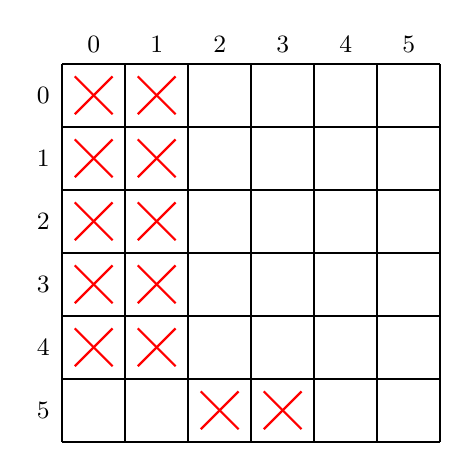
\begin{tikzpicture}[scale=0.8]
        \draw[thick] (0,0) grid (6,6);

        % Draw X marks
        \foreach \i/\j in {
            0/5, 1/5,
            0/4, 1/4,
            0/3, 1/3,
            0/2, 1/2,
            0/1, 1/1,
            2/0, 3/0
        } {
            \draw[red, thick] (\i+0.2,\j+0.2) -- (\i+0.8,\j+0.8);
            \draw[red, thick] (\i+0.8,\j+0.2) -- (\i+0.2,\j+0.8);
        }

        % Label rows and columns (optional)
        \foreach \i in {0,...,5} {
            \node at (\i+0.5,6.3) {\small \i};  % column labels
            \node at (-0.3,5.5-\i) {\small \i};  % row labels
        }
    \end{tikzpicture}
    \end{center}
    
\end{enumerate}
\end{document}